\section{Hyper-parameter selection and pilot results}
\label{app:pilot}
\paragraph{The $\beta$ pilot.} $\beta=0.1$ was chosen in October 2026 from $\{0, 0.1, 1\}$ in a pilot on DecisionBench that trained on 645 and tested on 430 of the README's 1,075 test rows, and in a learning-curve study whose test set overlapped the README slice. In that pilot $\beta=1$ kept about 80\% of the gain at 0.8B; in the learning-curve study it kept about a third. The historical grid also ran $\beta=1$ on the public menu and JevBench at 0.8B with results not included in its original summary: $\beta=1$ scored 0.584 against 0.590 for $\beta=0.1$ on the public menu and 0.548 against 0.517 on JevBench (released model 0.550). An independent reproduction of the historical DecisionBench study on another machine recovered the headline gain ($+10.4$ against $+10.2$) but not the KL pilot's gap ($\beta=0$: 0.566 against 0.571 for $\beta=0.1$, where the pilot had 0.536 against 0.567). The current grid did not retune this choice; $\beta=0.1$ is used throughout and the no-KL ablation has intervals.

\section{Reproducing the results}
\label{app:repro}
\path{experiments/peekaboo_remaining/run.py --grid v2} runs the whole grid: it reads every benchmark once through every model and caches the backbone features and the official records, replays each released model against its official prediction call, then runs every method and seed and writes \texttt{output\_v2/TABLES.md}. Finished steps are skipped, so the run can be resumed. \texttt{analysis.py} computes every interval, control and statistic in this paper from the per-row records, and \texttt{paper/make\_figures.py} produces every table, figure and number macro. The historical grid (\texttt{--grid v1}) and its results under \texttt{output/} are kept for comparison; its DecisionBench learning-curve study is run by \path{experiments/vega_policy/reproduce.py}.

\paragraph{How the grid was run.} The v2 plan was written for 540 steps. On one A40 the Laya encoder runs took 20 to 45 minutes each and the Laya head runs, which re-run the frozen encoder on every pass, more than an hour on the larger pools, so the plan was trimmed four times while the grid ran (repository commits \texttt{50ca000}, \texttt{73f3ed5}, \texttt{4dbf2e8}, \texttt{75a990e}): fewer encoder seeds, the Laya head arms cut to one pass, the realistic-feedback and no-KL arms cut to one seed outside DecisionBench, and no pooled variant. Steps that had already finished were kept, and the committed plan lists exactly the 314 steps that ran. No step was rerun to change a result; GPU out-of-memory failures were retried with the same code and seed.

\paragraph{Checks.} Replaying each released model on its cached inputs matches the official prediction call to $0$ for Vega and to $5\times10^{-5}$ for Laya (one question per forward pass, as Laya's own call runs it). The released models reproduce their README figures: Vega 0.8B and 4B on the public menu at $\accSmallBasePub$ and $\accBigBasePub$ against the README's 0.556 and 0.717, DecisionBench at $\accSmallBaseDb$ and $\accBigBaseDb$ against 0.509 and 0.633; Laya and laya-typed-decisions on typed-decisions at $\accLayaBaseTyped$ and $\accLayaTdTyped$ against 0.362 and 0.766. Results on the same seed differ across machines by up to 3 points for a single run (floating-point non-determinism in feature extraction and training kernels); these historical reruns are not an independent reproduction of the complete current grid.

\section{Training seed coverage}
\label{app:seeds}
\begin{table}[H]\centering\small
\caption{Independent training runs available in the current grid, counted from per-seed result files. Grouped methods have identical seed sets. A dash means not run. Early stopping reuses the labelled run; it is not another seed. Released models, TTT and historical head-only eight-pass runs are not included.}
\label{tab:seeds}
\setlength{\tabcolsep}{4pt}
\resizebox{\linewidth}{!}{\begin{tabular}{llrrrrrr}
\toprule
model & arms & public & JevBench & DecisionB. & typed-dec. & emotion & AG News \\
\midrule
Vega 0.8B & feedback and labelled, 8 / 1 passes & 3 & 3 & 3 & 3 & 3 & 3 \\
Vega 0.8B & logged and damaged feedback & -- & -- & 3 & 1 & 1 & -- \\
Vega 0.8B & no KL & 1 & 3 & 3 & 1 & 1 & 1 \\
Vega 0.8B & shipped adapters off & -- & -- & -- & 3 & -- & -- \\
Vega 4B & feedback and labelled, 8 / 1 passes & 3 & 3 & 3 & 3 & 3 & 3 \\
Vega 4B & logged and damaged feedback & -- & -- & 3 & 1 & 1 & -- \\
Vega 4B & no KL & 1 & 1 & 3 & 1 & 1 & 1 \\
Vega 4B & shipped adapters off & -- & -- & -- & 3 & -- & -- \\
Laya & encoder, feedback 8 / 1 and labelled 8 & 3 & 3 & 2 & 1 & 1 & -- \\
Laya & head, feedback and labelled 1 pass & 1 & 1 & 1 & 3 & -- & -- \\
\bottomrule
\end{tabular}}
\end{table}


\section{Per-task results}
\label{app:tasks}
\begin{table}[tbp]\centering\scriptsize
\caption{Accuracy on each of the 43 public tasks (mean over seeds). key: the early-stopped answer-key adapter / head; Pk8, Pk1: Peekaboo with eight passes, one pass; f-t: laya-typed-decisions; -enc: encoder unfrozen. $^*$ marks the two tasks with a construction artifact. Bold: the best method for that model on that task.}
\label{tab:tasks}
\setlength{\tabcolsep}{2pt}
\resizebox{\linewidth}{!}{\begin{tabular}{lrrrrrrrrrrrrrr}
\toprule
task & \multicolumn{5}{c}{Vega 0.8B} & \multicolumn{5}{c}{Vega 4B} & \multicolumn{4}{c}{Laya} \\
 & base & TTT & key & Pk8 & Pk1 & base & TTT & key & Pk8 & Pk1 & base & f-t & key-enc & Pk-enc \\
\midrule
aegis\_prompt\_safety & 0.50 & 0.50 & 0.64 & \textbf{0.64} & 0.57 & 0.60 & 0.60 & \textbf{0.79} & 0.74 & 0.73 & 0.37 & 0.43 & 0.68 & \textbf{0.70} \\
ag\_news & \textbf{0.97} & \textbf{0.97} & \textbf{0.97} & \textbf{0.97} & \textbf{0.97} & 0.95 & 0.95 & \textbf{0.97} & 0.95 & 0.97 & \textbf{0.98} & \textbf{0.98} & 0.97 & 0.97 \\
anli\_r3 & 0.28 & 0.28 & \textbf{0.39} & 0.37 & 0.32 & 0.35 & \textbf{0.52} & 0.43 & 0.40 & 0.39 & \textbf{0.43} & 0.40 & 0.42 & 0.42 \\
arc\_challenge & 0.48 & 0.48 & 0.44 & \textbf{0.50} & 0.48 & 0.80 & 0.80 & 0.80 & 0.81 & \textbf{0.83} & 0.28 & \textbf{0.37} & 0.34 & \textbf{0.37} \\
arc\_easy & \textbf{0.60} & \textbf{0.60} & 0.55 & 0.55 & 0.58 & 0.92 & 0.92 & \textbf{0.95} & 0.94 & 0.93 & 0.52 & 0.57 & \textbf{0.57} & 0.57 \\
banking77 & 0.68 & 0.68 & \textbf{0.72} & 0.66 & 0.62 & 0.73 & 0.73 & \textbf{0.74} & 0.69 & 0.69 & 0.42 & 0.40 & \textbf{0.48} & 0.37 \\
boolq & 0.75 & 0.75 & 0.76 & \textbf{0.82} & 0.79 & 0.82 & 0.82 & 0.84 & 0.84 & \textbf{0.91} & \textbf{0.87} & 0.85 & 0.78 & 0.83 \\
casehold & 0.35 & 0.35 & \textbf{0.49} & 0.46 & 0.42 & 0.55 & 0.55 & \textbf{0.63} & 0.61 & 0.63 & 0.38 & 0.38 & 0.38 & \textbf{0.45} \\
climate\_fever & 0.35 & 0.38 & \textbf{0.47} & 0.38 & 0.36 & 0.45 & 0.38 & \textbf{0.48} & 0.46 & \textbf{0.48} & 0.33 & \textbf{0.35} & 0.25 & 0.30 \\
clinc150\_oos & \textbf{0.68} & \textbf{0.68} & 0.62 & 0.62 & 0.61 & \textbf{0.92} & \textbf{0.92} & 0.83 & 0.78 & 0.83 & 0.00 & \textbf{0.32} & 0.00 & 0.00 \\
commonsenseqa & 0.35 & 0.35 & \textbf{0.41} & 0.38 & 0.35 & 0.53 & 0.53 & 0.59 & 0.59 & \textbf{0.60} & 0.45 & 0.45 & \textbf{0.47} & 0.45 \\
cruxeval\_output & 0.65 & 0.65 & \textbf{0.87} & 0.79 & 0.82 & 0.85 & 0.92 & \textbf{0.94} & 0.92 & \textbf{0.94} & 0.78 & 0.73 & 0.79 & \textbf{0.81} \\
dbpedia14 & 0.60 & \textbf{0.85} & 0.77 & 0.67 & 0.72 & 0.90 & \textbf{0.97} & 0.92 & 0.93 & 0.90 & 0.85 & 0.83 & 0.91 & \textbf{0.93} \\
emotion & \textbf{0.55} & \textbf{0.55} & 0.43 & 0.53 & 0.54 & \textbf{0.63} & 0.45 & 0.52 & 0.52 & 0.61 & \textbf{0.57} & \textbf{0.57} & 0.53 & 0.53 \\
enron\_spam & \textbf{1.00} & \textbf{1.00} & \textbf{1.00} & 0.99 & \textbf{1.00} & \textbf{1.00} & \textbf{1.00} & \textbf{1.00} & \textbf{1.00} & 0.99 & 0.92 & 0.90 & \textbf{0.93} & 0.92 \\
glue\_rte & \textbf{0.62} & \textbf{0.62} & 0.61 & \textbf{0.62} & 0.58 & 0.87 & 0.85 & 0.87 & 0.86 & \textbf{0.89} & \textbf{0.83} & 0.82 & 0.82 & 0.80 \\
hellaswag & 0.25 & 0.25 & 0.27 & \textbf{0.32} & 0.28 & \textbf{0.65} & \textbf{0.65} & 0.58 & 0.53 & 0.59 & 0.37 & 0.37 & 0.39 & \textbf{0.39} \\
jailbreak\_cls & \textbf{0.98} & \textbf{0.98} & \textbf{0.98} & 0.97 & 0.96 & \textbf{1.00} & \textbf{1.00} & 0.99 & 0.98 & 0.99 & 0.98 & 0.98 & 0.98 & \textbf{0.99} \\
ledgar & 0.33 & 0.33 & \textbf{0.59} & 0.40 & 0.39 & 0.63 & 0.63 & 0.63 & 0.63 & \textbf{0.66} & 0.25 & 0.18 & \textbf{0.47} & 0.33 \\
massive\_intent\_en & 0.38 & 0.38 & \textbf{0.53} & 0.43 & 0.43 & 0.60 & 0.60 & \textbf{0.64} & 0.59 & 0.60 & 0.38 & 0.42 & \textbf{0.47} & 0.38 \\
medmcqa & 0.18 & 0.18 & 0.19 & 0.28 & \textbf{0.30} & 0.48 & 0.48 & \textbf{0.49} & \textbf{0.49} & 0.48 & \textbf{0.35} & \textbf{0.35} & 0.32 & 0.31 \\
medqa\_usmle & 0.31 & 0.31 & 0.27 & 0.29 & \textbf{0.31} & 0.51 & 0.51 & \textbf{0.55} & 0.53 & \textbf{0.55} & 0.20 & \textbf{0.29} & 0.23 & 0.28 \\
mmlu & \textbf{0.37} & \textbf{0.37} & 0.32 & 0.32 & 0.31 & \textbf{0.73} & \textbf{0.73} & 0.63 & 0.57 & 0.61 & 0.25 & \textbf{0.35} & 0.31 & 0.32 \\
mmlu\_pro & 0.20 & 0.13 & 0.16 & 0.21 & \textbf{0.24} & \textbf{0.40} & \textbf{0.40} & 0.39 & \textbf{0.40} & 0.38 & \textbf{0.18} & \textbf{0.18} & \textbf{0.18} & 0.18 \\
openbookqa & \textbf{0.58} & \textbf{0.58} & 0.53 & 0.54 & 0.58 & \textbf{0.83} & \textbf{0.83} & 0.79 & 0.78 & 0.79 & 0.40 & 0.48 & \textbf{0.53} & 0.49 \\
prompt\_injections & 0.75 & \textbf{0.96} & 0.87 & 0.85 & 0.76 & 0.85 & \textbf{0.96} & 0.82 & 0.89 & 0.90 & 0.65 & 0.60 & 0.81 & \textbf{0.84} \\
pubmedqa$^*$ & 0.13 & \textbf{0.58} & 0.54 & 0.55 & 0.54 & 0.40 & \textbf{0.62} & 0.60 & 0.56 & 0.55 & 0.53 & 0.55 & \textbf{0.64} & 0.61 \\
race\_middle & 0.60 & 0.60 & 0.54 & \textbf{0.61} & 0.57 & 0.82 & \textbf{0.90} & 0.82 & 0.81 & 0.82 & 0.58 & 0.52 & \textbf{0.59} & 0.53 \\
sciq & 0.73 & 0.73 & 0.67 & 0.72 & \textbf{0.76} & 0.92 & 0.92 & \textbf{0.95} & 0.94 & 0.93 & 0.52 & 0.55 & \textbf{0.56} & 0.52 \\
superglue\_cb & 0.67 & 0.69 & 0.68 & \textbf{0.75} & 0.70 & 0.82 & \textbf{0.87} & 0.81 & 0.78 & 0.82 & \textbf{0.87} & 0.84 & 0.83 & 0.79 \\
toxic\_chat\_jailbreak & \textbf{0.98} & \textbf{0.98} & 0.96 & 0.91 & 0.92 & 0.92 & 0.92 & \textbf{0.95} & \textbf{0.95} & 0.94 & 0.83 & \textbf{0.90} & 0.84 & 0.87 \\
toxic\_chat\_toxicity & \textbf{0.95} & 0.93 & 0.93 & 0.90 & 0.92 & \textbf{1.00} & 0.98 & 0.98 & 0.98 & 0.98 & \textbf{0.97} & \textbf{0.97} & 0.94 & 0.92 \\
trec\_coarse & 0.53 & 0.68 & \textbf{0.72} & 0.61 & 0.60 & 0.77 & \textbf{0.88} & 0.83 & 0.77 & 0.75 & 0.57 & 0.52 & \textbf{0.89} & 0.56 \\
truthfulqa\_mc1$^*$ & 0.34 & 0.34 & \textbf{0.77} & 0.71 & 0.53 & 0.64 & 0.64 & \textbf{0.73} & 0.72 & 0.65 & 0.16 & 0.24 & \textbf{0.41} & 0.38 \\
tweet\_hate & \textbf{0.65} & 0.63 & 0.62 & 0.61 & 0.53 & \textbf{0.68} & 0.60 & 0.57 & 0.61 & 0.59 & \textbf{0.73} & 0.72 & 0.64 & 0.67 \\
tweet\_irony & \textbf{0.78} & 0.60 & 0.71 & 0.67 & 0.70 & \textbf{0.78} & \textbf{0.78} & 0.74 & 0.73 & 0.71 & \textbf{0.78} & 0.74 & 0.71 & 0.73 \\
tweet\_offensive & 0.80 & 0.80 & 0.81 & 0.80 & \textbf{0.81} & 0.78 & 0.78 & \textbf{0.85} & 0.78 & 0.80 & 0.69 & 0.71 & \textbf{0.79} & 0.78 \\
tweet\_sentiment & 0.44 & 0.44 & 0.45 & \textbf{0.50} & 0.46 & \textbf{0.58} & \textbf{0.58} & 0.49 & 0.56 & 0.49 & \textbf{0.56} & 0.49 & 0.45 & 0.45 \\
tweet\_stance\_abortion & 0.36 & 0.45 & 0.48 & \textbf{0.58} & 0.40 & \textbf{0.55} & 0.49 & 0.48 & 0.31 & 0.45 & 0.31 & 0.31 & 0.38 & \textbf{0.44} \\
unfair\_tos & \textbf{0.74} & 0.65 & 0.56 & 0.57 & 0.54 & \textbf{0.88} & 0.70 & 0.82 & 0.73 & 0.71 & \textbf{0.88} & 0.84 & 0.61 & 0.61 \\
vitaminc & 0.47 & 0.47 & \textbf{0.54} & 0.47 & 0.53 & 0.62 & 0.62 & 0.63 & 0.61 & \textbf{0.64} & 0.43 & 0.33 & \textbf{0.66} & 0.62 \\
winogrande & 0.50 & 0.50 & \textbf{0.52} & 0.49 & 0.51 & 0.58 & 0.58 & 0.62 & \textbf{0.63} & \textbf{0.63} & 0.53 & 0.50 & 0.53 & \textbf{0.57} \\
yelp\_stars & 0.50 & 0.50 & \textbf{0.59} & 0.49 & 0.45 & \textbf{0.58} & \textbf{0.58} & 0.52 & 0.47 & 0.52 & 0.28 & 0.37 & \textbf{0.59} & 0.38 \\
\bottomrule
\end{tabular}}
\end{table}

\begin{table}[tbp]\centering\scriptsize
\caption{DecisionBench per task (25 test rows each): accuracy of the released model and gain in points of Peekaboo (8 passes), the answer-key adapter and TTT (0.8.0 rule). $^*$: tasks with a construction artifact.}
\label{tab:tasks_db}
\setlength{\tabcolsep}{3pt}
\begin{tabular}{lrrrrrrrr}
\toprule
task & \multicolumn{4}{c}{Vega 0.8B} & \multicolumn{4}{c}{Vega 4B} \\
 & base & Pk & key & TTT & base & Pk & key & TTT \\
\midrule
tool-action-impact & 0.68 & +1 & +1 & +4 & 0.60 & +7 & +15 & +12 \\
agent-skill-ranking & 0.40 & +16 & +8 & +0 & 0.64 & +1 & +0 & +0 \\
tool-call-routing & 0.52 & +0 & -5 & +0 & 0.52 & +5 & +0 & +0 \\
tool-safety-gate & 0.32 & +61 & +64 & +60 & 0.96 & -3 & +4 & +0 \\
runtime-outcome-verification & 0.48 & -3 & -3 & +4 & 0.44 & +3 & +0 & +8 \\
browser-action-selection & 0.52 & +8 & +16 & +0 & 0.76 & -3 & -9 & +0 \\
browser-target-selection & 0.12 & +7 & +5 & +0 & 0.32 & +3 & -5 & +0 \\
codebase-result-ranking & 0.48 & +7 & -3 & +0 & 0.52 & +4 & -7 & +0 \\
semantic-line-match & 0.96 & +0 & -5 & +0 & 0.96 & -1 & -5 & -4 \\
agent-readiness-assessment & 0.72 & +8 & +12 & +0 & 0.80 & +11 & +11 & +0 \\
agent-call-retention & 0.92 & +1 & -4 & -4 & 0.68 & +25 & +32 & +28 \\
agent-result-retention & 1.00 & +0 & +0 & +0 & 0.92 & +8 & +8 & +0 \\
database-row-classification & 0.44 & +7 & -5 & +0 & 0.40 & +4 & -3 & +0 \\
relevance\_score & 0.36 & -7 & +5 & +8 & 0.52 & -8 & -8 & -4 \\
claim-evidence-verification & 0.52 & +8 & +5 & -4 & 0.80 & +5 & +0 & -12 \\
trading-action-selection & 0.40 & +5 & -3 & +0 & 0.36 & +9 & +9 & +0 \\
finqa-numerical-reasoning$^*$ & 0.16 & +39 & +49 & +0 & 0.44 & +13 & +21 & +0 \\
route & 0.40 & +4 & +8 & +0 & 0.76 & -3 & -7 & +0 \\
game-goal-selection & 0.40 & +17 & +11 & +0 & 0.52 & +7 & +12 & +0 \\
platformer-control-selection & 0.16 & +11 & +5 & +4 & 0.36 & -4 & +8 & +4 \\
strategy-command-selection & 0.16 & +17 & +19 & +0 & 0.32 & +3 & +8 & +0 \\
route & 0.76 & -9 & +0 & +0 & 0.80 & +1 & +0 & +0 \\
home-alert-triage & 0.44 & +37 & +40 & +0 & 0.64 & +24 & +23 & +0 \\
graph-edge-selection & 0.32 & +19 & +20 & +0 & 0.80 & +7 & -4 & +0 \\
workflow\_decision & 0.48 & +11 & +8 & +20 & 0.84 & +4 & -1 & +8 \\
workflow\_decision & 0.72 & +3 & +3 & +4 & 0.88 & -4 & -4 & -12 \\
folio-logical-inference & 0.44 & -9 & -9 & -24 & 0.60 & -5 & -9 & -24 \\
musique-evidence-sufficiency & 0.60 & -8 & -1 & -24 & 0.60 & -3 & -7 & -24 \\
musique-multihop-answer & 0.52 & +27 & +33 & +0 & 0.40 & +27 & +33 & +0 \\
contains\_threat$^*$ & 0.76 & +24 & +24 & +0 & 1.00 & +0 & +0 & +0 \\
toxicity\_severity$^*$ & 0.20 & +49 & +48 & +48 & 0.20 & +51 & +49 & +24 \\
bounded\_value & 0.88 & +1 & +4 & +0 & 1.00 & +0 & -3 & +0 \\
canonical\_entity & 0.72 & +21 & +21 & +0 & 0.96 & -4 & -5 & +0 \\
drone-tactical-action & 0.16 & +36 & +52 & +0 & 0.64 & +3 & +11 & +0 \\
robot-skill-selection & 0.40 & +7 & +13 & +0 & 0.48 & +1 & -7 & +0 \\
search-plan-routing & 0.56 & +19 & +15 & +0 & 0.72 & +11 & +4 & +0 \\
social-post-filtering & 0.56 & +16 & +16 & +12 & 0.84 & +4 & +1 & -12 \\
tool\_route & 0.84 & +4 & +1 & +0 & 0.92 & +0 & +0 & +0 \\
code-change-risk & 0.44 & +16 & +21 & +0 & 0.52 & +8 & +12 & -4 \\
tax-document-page-classification & 0.04 & +1 & +12 & +0 & 0.12 & +0 & +3 & +0 \\
patent\_section & 0.40 & -4 & -1 & -12 & 0.28 & +8 & +16 & +4 \\
relevance & 0.76 & -4 & +4 & -12 & 0.76 & +4 & +0 & +8 \\
dom-ad-detection & 0.76 & +21 & +24 & +8 & 0.76 & +24 & +24 & +16 \\
\bottomrule
\end{tabular}
\end{table}


\begin{figure}[H]\centering
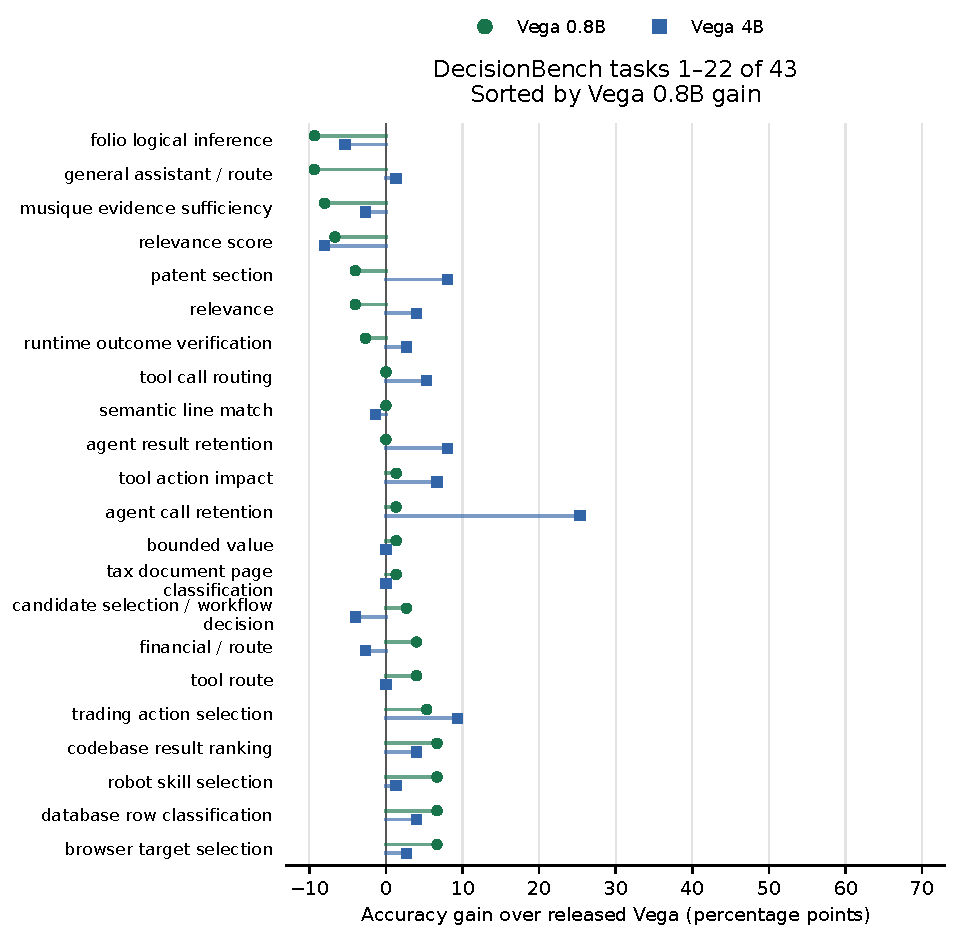
\includegraphics[width=\linewidth]{tasks_db.pdf}
\caption{DecisionBench task gains, tasks 1--22 of 43, sorted by the Vega 0.8B gain. Horizontal labels identify each task; circles are Vega 0.8B and squares Vega 4B. Endpoints show mean accuracy gains over the released model; lines connect each point to zero and are not confidence intervals. Each task has 25 test rows. The second panel is Figure~\ref{fig:tasks_db_more}; both use the same horizontal scale. $^*$ marks identified benchmark shortcuts.}
\label{fig:tasks_db}
\end{figure}

\begin{figure}[H]\centering
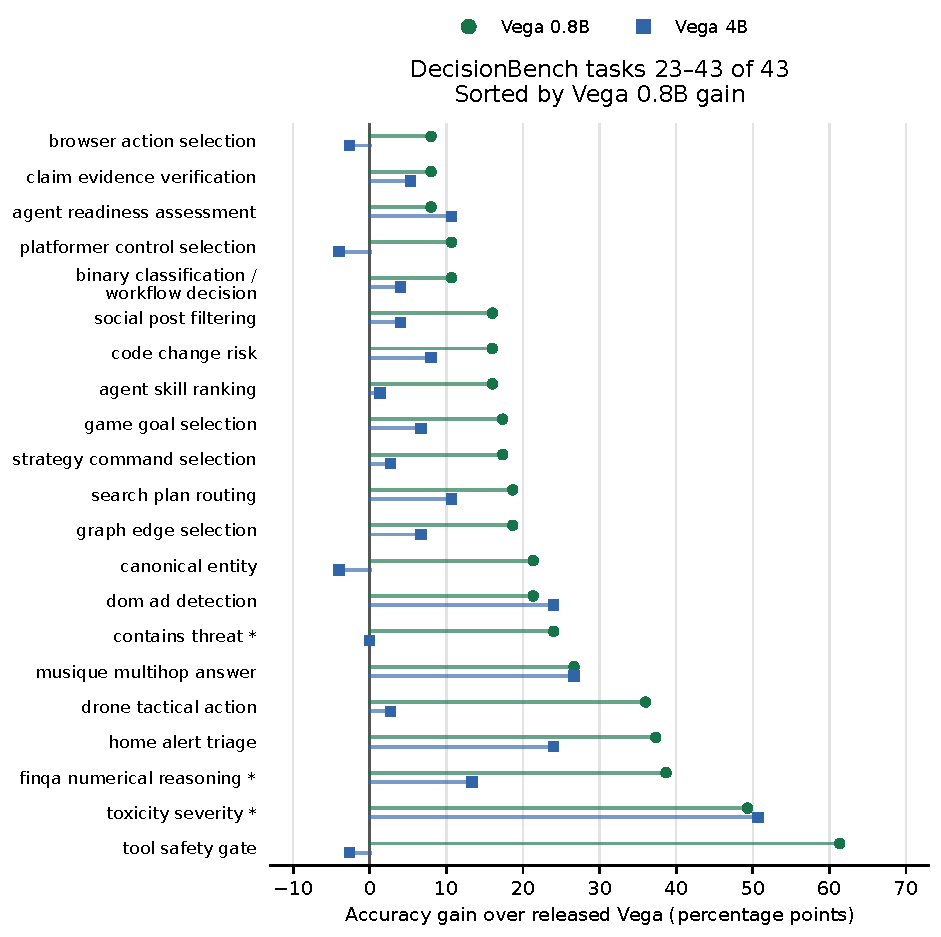
\includegraphics[width=\linewidth]{tasks_db_more.pdf}
\caption{DecisionBench task gains continued, tasks 23--43 of 43. Order, symbols and horizontal scale match Figure~\ref{fig:tasks_db}. $^*$ marks identified benchmark shortcuts.}
\label{fig:tasks_db_more}
\end{figure}
\FloatBarrier

\section{Hyper-parameters}
\begin{table}[H]\centering\small
\begin{tabular}{lp{12.5cm}}
\toprule
add-on, Vega & gated LoRA, rank 8, on seven engine layers (\texttt{vegaml.attach\_adapter}); 409k / 857k parameters \\
add-on, Laya & trainable copy of type embedding, 2-layer decision head and scorer (26.5M); encoder frozen, or a trained copy (``encoder unfrozen'', 421M in all) \\
optimiser & Adam; lr $10^{-3}$ (Vega adapter), $10^{-4}$ (Laya head), $2.5\times10^{-5}$ (Laya encoder); grad-norm clip 1.0 \\
schedule & 8 passes (or 1), batches of 32 (encoder: micro-batches of 8, one update per 32 rows) \\
reward & $r = \mathbf{1}[\text{sampled answer} = \text{gold}]$; baseline $b \leftarrow 0.9\,b + 0.1\,\bar r$, $b_0 = 0.5$ \\
KL term & $\beta = 0.1$ for every trained arm (ablation: 0) \\
answer-key arms & cross-entropy on the gold answer, same KL term; early stopping picks the epoch with the best argmax accuracy on the calibration rows \\
logged arms & best answer: $-r\log\pi(a) - (1-r)\log(1-\pi(a))$ on the released model's argmax, rated once; sampled: clipped importance weights (cap 10) on one answer sampled from the released model \\
honesty fix & $T$ on a 61-point log grid in $[0.25, 32]$, maximising the Bernoulli likelihood of verdicts on sampled answers from the calibration rows; label arms: NLL temperature scaling on the same rows \\
switch & keep the add-on if its best answers are right more often than the released model's on the calibration rows \\
label prior & one log-offset per (task, option text); same loop, lr from $\{10^{-3}, 10^{-2}, 3\times10^{-2}, 10^{-1}\}$ chosen on the calibration rows' verdicts \\
splits & feedback rows 80\,/\,20 train\,/\,calibration per task by a fixed permutation; JevBench 5-fold by paraphrase group, calibration fifth by paraphrase group \\
intervals & 2,000 bootstrap replicates resampling seeds and row clusters; Holm within families; non-inferiority margin 2 points \\
seeds & 0, 1, 2 \\
\bottomrule
\end{tabular}
\end{table}
